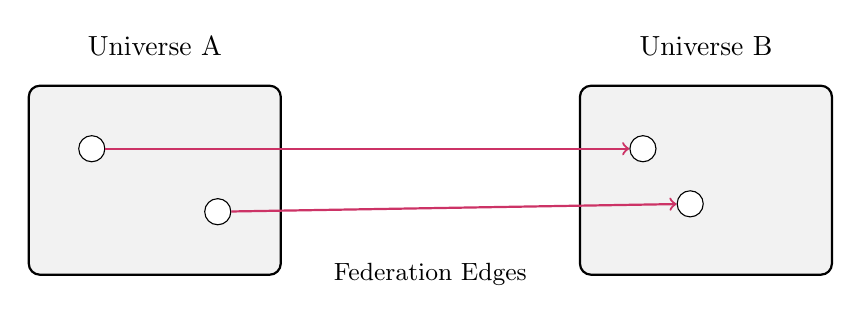
\begin{tikzpicture}[
    uni/.style={rectangle, draw=black, thick, fill=gray!10, rounded corners, minimum width=3.2cm, minimum height=2.4cm},
    link/.style={->, thick, draw=purple!80},
    node/.style={circle, draw=black, fill=white, minimum size=5pt}
]

\node[uni] (UA) at (0,0) {};
\node[uni] (UB) at (7,0) {};

\node at (0,1.7) {Universe A};
\node at (7,1.7) {Universe B};

\node[node] (A1) at (-0.8,0.4) {};
\node[node] (A2) at (0.8,-0.4) {};
\node[node] (B1) at (7-0.8,0.4) {};
\node[node] (B2) at (7-0.2,-0.3) {};

\draw[link] (A1) -- (B1);
\draw[link] (A2) -- (B2);

\node at (3.5,-1.2) {\small Federation Edges};

\end{tikzpicture}